\documentclass[usletter]{article}
\usepackage{graphicx}
\usepackage{amsfonts}
\usepackage{amsthm}
\usepackage{amsmath}
\usepackage{amssymb}
\usepackage{hyperref}
\hypersetup{
    colorlinks=true,
    linkcolor=blue,
    filecolor=magenta,      
    urlcolor=cyan,
}
\usepackage{scribe}
\usepackage[margin=1.5in]{geometry}

\begin{document}

    
\makeheader{Sanket Kanjalkar, Yunqi Li}                              % your name
           {October 09, 2019}                          % lecture date
           {11}                                       % lecture number
           {Fully Homomorphic Encryption I}  % lecture title

\newcommand{\floor}[1]{\left\lfloor #1 \right\rfloor}
\newcommand{\ceil}[1]{\left\lceil #1 \right\rceil}

Informally, a cryptosystem that supports arbitrary computation on ciphertexts is known as fully homomorphic encryption (FHE)\cite{wiki}. Throughout the course, we have studied encryption schemes for information transfer from one party to another party. However, if we were to compute on data using our traditional encryption schemes, it would require that data must be decrypted before it can be analyzed or manipulated. Naturally, one asked the question whether it is possible to compute on Encrypted Data. That is, it should be possible to compute a known function on encrypted data without having access to the secret key. 

Such an FHE scheme can be used for privacy-preserving outsourced storage and computation. In today's lecture, we will see what is fully homomorphic encryption (FHE) scheme and how to build an FHE scheme. We will also look at intuitive ways to construct FHE for addition and multiplication.

\begin{fact}
LWE is the only way we know to do fully homomorphic encryption as of Sept 2019. 
\end{fact}
           
\section{Recap}

We provide a quick primer on the notation used in this section. 
\begin{itemize}
    \item All values which are bolded like $\pmb{s}, \pmb{a}$ are vectors where bolded Captial $\pmb{A}$ is a matrix.
    \item All values which in simple like $q, e$ are scalars. All scalars apart from field modulas $q$ are in field $Z_q$.
    \item The values $\pmb{a}, \pmb{A}$ are public value seen by all parties, \pmb{s} is secret value and $e$, $\pmb{e}$ are errors
\end{itemize}


Before stepping into how to build LWE-based FHE schemes, let's briefly recap how to build a private and public encryption scheme with the LWE problem.
Desisional LWE is the problem where given a matrix $A_{n,m}$, and a vector $b_m$, determining whether or not these are results vector of some instance of an LWE problem OR whether the vector $b_m$ was simply 
drawn from sampling values uniformly randomly from $Z^{m}_{q}$. 
\begin{definition}
\textbf{\textit{Decisional $LWE{n,m,q,\mathcal{X}}$}} : For all non-uniform probabilistic polynomial time adversary $\mathcal{A}$
$$|\underset{\substack{
\pmb{s}\leftarrow \mathbb{Z}_q^{n\times1}\\
\pmb{A}\leftarrow\mathbb{Z}_q^{n\times m}\\
\pmb{e}\leftarrow \mathcal{X}^m}}{Pr}
[\mathcal{A}(\pmb{A},\pmb{s}^T\pmb{A}+\pmb{e}^T)=1]
-\underset{\substack{\pmb{A}\leftarrow\mathbb{Z}_q^{n\times m}\\
\pmb{b}\leftarrow\mathbb{Z}_q^m}}{Pr} 
[\mathcal{A}(\pmb{A},\pmb{b})=1]|=negl(n)$$
where $q$ is a prime within $O(2^n)$, $m=O(n\log q)$ and norm $\parallel \pmb{e}\parallel=\omega(\log n)$. Where $\omega(f(n))$ means that 
$e$ should be greater than $f(n)$ assymptotically.
\end{definition}


Next, we revise the secret key encryption (SKE) built with LWE which has $m=1$. The secret key here is a vector $\pmb{s} \in \mathbb{Z}_q^n$. We refer to the previous lecture for the definition of SKE and only give an instantiation of one using LWE.

$$KeyGen(1^n): \pmb{s}\leftarrow\mathbb{Z}_q^n$$
$$\underset{\substack{
\pmb{s}\leftarrow \mathbb{Z}_q^{n\times1}\\
\pmb{a}\leftarrow\mathbb{Z}_q^{n\times 1}\\
\pmb{e}\leftarrow \mathcal{X}}}{Enc}(\pmb{s},\mu\in\{0,1\}): (\pmb{a}, (b = \pmb{s}^T\pmb{a}+e+\mu\lfloor\frac{q}{2}\rfloor)\mod q)$$


$$Dec(\pmb{s},\pmb{a},b): b-\langle\pmb{s}^T,\pmb{a}\rangle=(e+\mu\lfloor\frac{q}{2}\rfloor) \mod q =   
  \begin{cases}
    0 & \text{if $b - \pmb{s}^T\pmb{a}$ mod q}  \in [\frac{-q}{4} \frac{q}{4} ] \\% - \pmb{s}^T\pmb{a} mod q  \[\floor{-q}{4} \floor{q}{4}\]$} \\
    1 & \text{if $b - \pmb{s}^T\pmb{a}$ mod q}  \in [\frac{q}{4} \frac{3q}{4} ]%  \[\floor{q}{4} \floor{3*q}{4}\]$}
  \end{cases}$$
  

LWE can also be used to build public key encryption(PKE) with public key $pk = (\pmb{A}, \pmb{b}^T=\pmb{s}^T\pmb{A}+\pmb{e}^T))$ and secret key $sk$. Just as before, interested reader can look at the definition of PKE in  and here we only an instantiation of the scheme using LWE.
$$\underset{\substack{
\pmb{A}\leftarrow\mathbb{Z}_q^{n\times m}\\
\pmb{a}\leftarrow\mathbb{Z}_q^{n\times 1}\\
\pmb{e}\leftarrow\mathcal{X}^m}}{KeyGen}(1^n): (sk=\pmb{s},pk=(\pmb{A}, \pmb{b}^T=\pmb{s}^T\pmb{A}+\pmb{e}^T))$$


$$\underset{\substack{
\pmb{r}\leftarrow\{0,1\}^m\\}}{Enc}(pk = (\pmb{A}, \pmb{b}^T) ,\mu\in\{0,1\}): (\pmb{c_1}=\pmb{A}\pmb{r}, c_2=(\pmb{b}^T\pmb{r}+\mu\lfloor\frac{q}{2}\rfloor)\mod q)$$

$$Dec(sk=\pmb{s},(\pmb{c_1},c_2)): c_2-\pmb{s}^T\pmb{c_1}=\pmb{e}^T\pmb{r}+\mu\lfloor\frac{q}{2}\rfloor \mod q =  \begin{cases}
    0 & \text{if $c_2-\pmb{s}^T\pmb{c_1}$ mod q}  \in [\frac{-q}{4} \frac{q}{4} ] \\% - \pmb{s}^T\pmb{a} mod q  \[\floor{-q}{4} \floor{q}{4}\]$} \\
    1 & \text{if $c_2-\pmb{s}^T\pmb{c_1}$ mod q}  \in [\frac{q}{4} \frac{3q}{4} ]%  \[\floor{q}{4} \floor{3*q}{4}\]$}
  \end{cases}$$
    
\begin{remark}
Generally, we want the noise $\pmb{e}$ introduced to the equations that are sampled from a distribution with zero mean and low standard variation. For the correctness of the encryption scheme, we will require that the noise distribution makes noise bound $\parallel e\parallel\leq q/4$ with high probability. As shown in the above decryption scheme, if the norm of noises is bounded by $q/4$, the boundary between the case $\mu=1$ and $\mu=0$ is very clear and the probability that decryption algorithm giving the wrong plaintext is very slow. In practice, $\mathcal{X}$ is usually a discrete Gaussian distribution over $\mathbb{Z}_q$. With Gaussian distribution that has to mean $\mu=0$ and standard variation $\sigma$ to be very small, according to its probability density function:
$$f(x)=\frac{1}{\sqrt{2\pi\sigma}}e^{-\frac{x^2}{2\sigma^2}}$$
we can get that the error bound to go beyond $q/4$ is negligible when $\sigma\ll q/4$.
\end{remark}

\begin{remark}
We also recall that parameters $e$, $\pmb{e}$ in both of the schemes above are neither in the public key nor in the secret key! That is neither the Encryption algorithms or the Decryption algorithms use it. But, it is also important for the security of the above schemes that errors are not known to other parties even though it is not a part of the secret key.
\end{remark}

\section{Fully Homomorphic Encryption (FHE)}

Let us consider the scenario shown in \ref{com}. A client has a secret value of $x$. The client wants the server to do some computation on $x$ without revealing what $x$ is. To accomplish the following we do we follow the below protocol: First, a ciphertext $ct=Enc(x)$ is sent to the server along with the desired function $f$. The server then computes a new ciphertext $ct^*=Enc(f(x))$ by evaluating $x$ on another function $g$ which is publicly computable from $f$. After receiving $ct^*$ from the server, the client can use its secret key $sk$ to get the desired result of $f(x)$. Note that in the following example, the server learns the function $f$ so it is aware of what computation is taking place, but cannot figure the values underneath. 

Fully Homomorphic Encryption refers to an extension of Encryption scheme with additional keywords \texttt{Fully} and \texttt{Homomorphic}.
\texttt{Homomorphic} in FHE refers to homomorphism in mathematics: the encryption and decryption functions can be thought of as homomorphisms between plaintext and ciphertext domains. \texttt{Fully} refers to the fact that we can evaluate any function. There is another variant called \texttt{Levelled} Homomorphic encryptions where we restrict ourselves to evaluating only functions with certain complexity(depth). 

Even though the Fully Homomorphic encryption scheme is our actual goal, in practice we also consider a simplification leveled fully homomorphic encryption scheme. Leveled FHE does not allow us to compute arbitrary functions $f$ but only functions with a known depth $d$. Informally, when we already know what is the most complex(in terms of depth of the arithmetic circuit) and use that in the construction of our FHE scheme.


\begin{figure}[!htbp]
\begin{center}
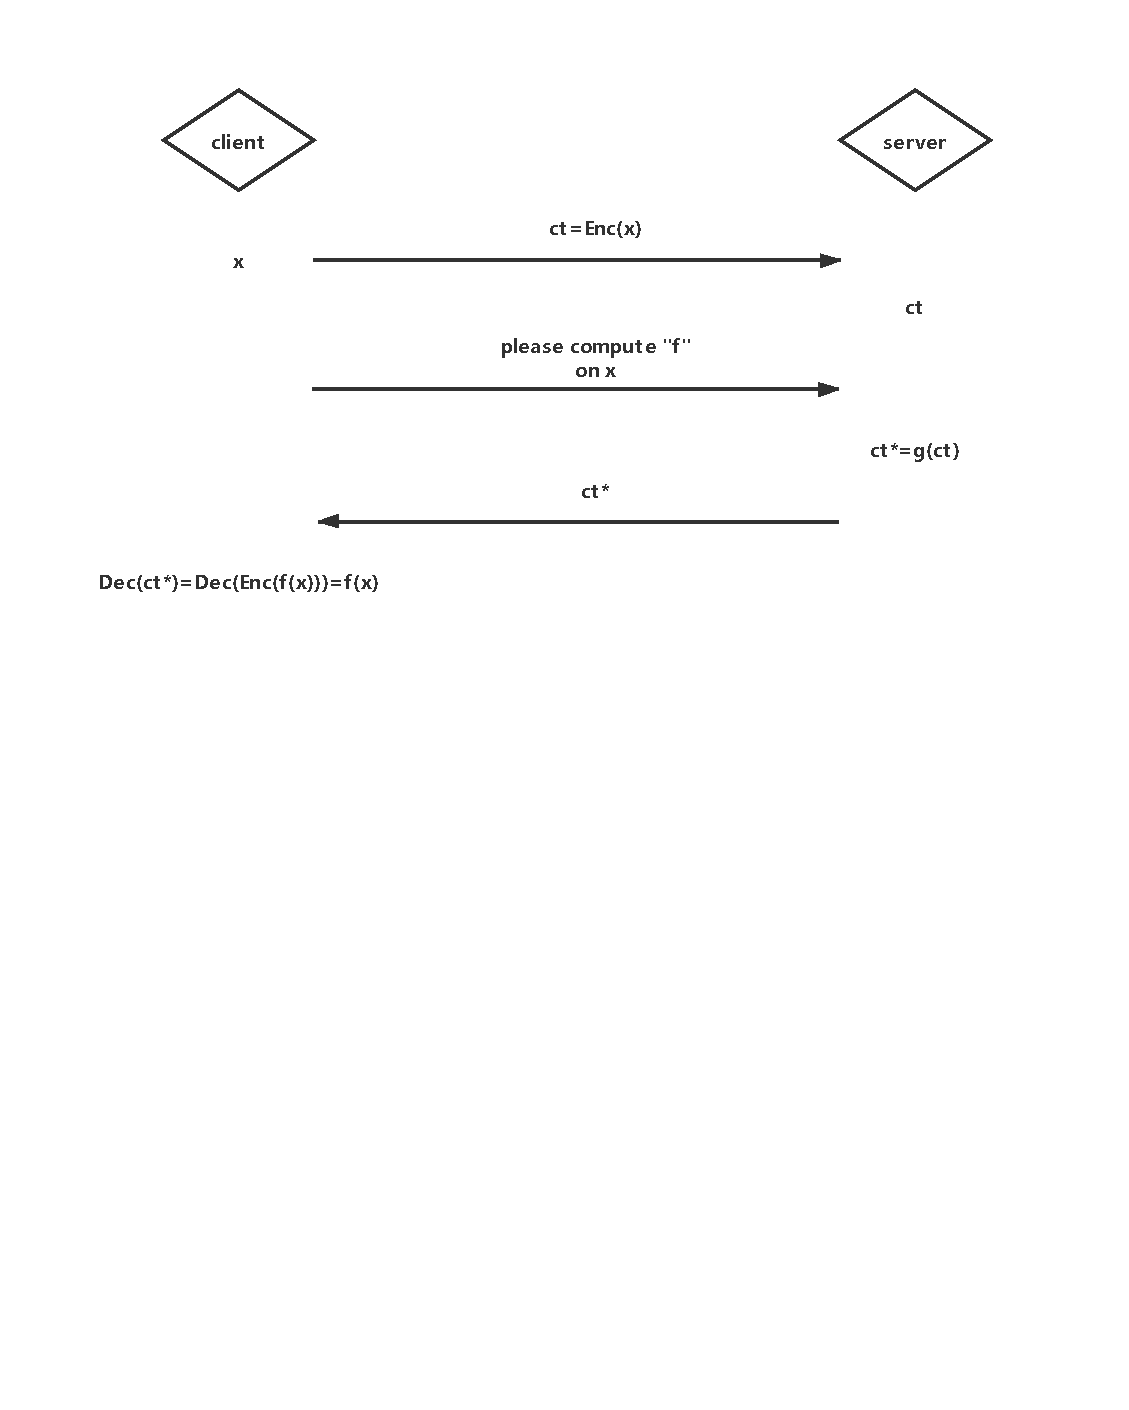
\includegraphics[width=0.9\textwidth]{client-server.pdf}
\end{center}
\caption{Outsourced Computation}
\label{com}
\end{figure}

 FHE allows operations and analysis of encrypted data without revealing the original one, which removes the privacy barriers in several real-life applications. 

\begin{definition} Let $\mathcal{C}$ be a class of circuits where for each $f\in\mathcal{C}$, $f:\{0,1\}^n \rightarrow \{0,1\}$. An encryption scheme $(KeyGen, Enc, Dec, Eval)$ is \textbf{$\mathcal{C}$-homomorphic} if $\forall f\in \mathcal{C}$, all ciphertexts $ct_1, \dots, ct_n$, $Eval(f, ct_1,\dots,ct_n)=ct^*$ such that if  $\forall i$, $\exists m_i, r_i$ s.t. $ct_i=Enc(m_i;r_i)$, then $Dec_{sk}(ct^*)=f(m_1,\dots,m_n)$ and the scheme is IND-CPA secure.
\end{definition}
At a high level, given ciphertexts $ct_1,\dots,ct_n$ that encrypt $m_1,\dots,m_n$, FHE should allow anyone to output a ciphertext  $ct^*$ that encrypts $f(m_1,\dots,m_n)$ for any desired function $f$ by evaluating another function $g$ which is publicly computable from $f$. Thus, the key holder could use the secret key $sk$ to decrypt $ct^*$ and get the result of $f(m_1,\dots,m_n)$. 

Note that each function $f:\{0,1\}^n\rightarrow\{0,1\}^k$ can be split into $f_1,\dots,f_k$ where $\forall i$, $f_i:\{0,1\}^n\rightarrow\{0,1\}$ and also we can generalized the definition by regulating the input length of circuits in $\mathcal{C}$ from $n$ to $poly(n)$.



\begin{remark}
    In the Leveled homomorphic setting, it is possible to hide the function $f$ being evaluated under a Universal function evaluator. That is if we know the bound of the number of gates and depth of the circuits being evaluated, we can use the function $f$ as an argument to another universal function evaluator.
    $$Eval(U, f, args) = f(args)$$
\end{remark}

\section{Construction of Fully Homomorphic Encryption:}
As described previously, FHE is an encryption scheme \texttt{(KeyGen, Enc, Dec)} 
with an additional algorithm called \texttt{Eval}. In particular, we want to construct such a \texttt{Eval} namely for two operations, Addition, and Multiplication. Constructing such an FHE scheme which must work for \textbf{all} functions $f$ might seem like a daunting task, 
but can use the following fact to ease our task.
\begin{fact}
It turns out that all functions can be expressed by arithmetic circuits consisting
of only addition and multiplication gates. Therefore, we only implement our FHE operations for addition and Multiplication. We can recursively compute every gate in the arithmetic circuit homomorphically to get the output of the function. 
\end{fact}

\begin{definition}
An arithmetic circuit over a field $\mathbb{Z}_q$ is a directed
acyclic graph whose vertices are called gates. Gates of incoming degree $0$ are inputs to
the circuit. All other gates are labeled $+$ or $x$. 
\end{definition}
We usually consider arithmetic circuits with fan-in $2$, in which case all of the $+$ and $\times$ gates have in-degree $2$.

Let us start with the simplest possible way to build an FHE for the addition operation. 
For simplicity, let us consider that we want to single-bit numbers and output a single bit number. This is equivalent to implementing the XOR operation. 

\section{FHE: Addition Operation}

\begin{remark}
    It is important to know that the symbols $+$ are being used interchangeably with $\oplus$. When we are saying addition, we XORing the messages. We maintain this notion to be consistent with the literature in FHE.
\end{remark}

Consider an encryption of message $\mu_1$ under the public key ($\pmb{s}^{T}\pmb{A} + \pmb{e}^{T}, \pmb{A}$). We call 
$\pmb{s}^{T}\pmb{A} + \pmb{e}^{T}$ as $\pmb{b}$. One intuitive naive way to implementing addition might be addition of ciphertexts.

\begin{claim}
    $c_1 + c_2$ is an encryption of $\mu_1 + \mu_2$
\end{claim}

$$c_1 = ( \pmb{Ar_1}, \pmb{br_1} + \mu_1\floor{\frac{q}{2}} )$$
$$c_2 = ( \pmb{Ar_2}, \pmb{br_2} + \mu_2\floor{\frac{q}{2}} )$$
$$c_{add} = c_1 + c_2 = ( \pmb{A}(\pmb{r_1} + \pmb{r_2}), \pmb{b}(\pmb{r_1} +\pmb{r_2}) + (\mu_1 + \mu_2)\floor{\frac{q}{2}} )$$

It is possible to extend this to multi-bit XOR outputs by simply repeating the circuit multiple times. However, it would only help in computing XOR for two $k$ bit numbers. 
Let us try to decrypt the ciphertext $c_{add}$ and check what it decrypts to:

\begin{align*}
Dec(sk,c_{add})
&= \pmb{b}(\pmb{r_1} +\pmb{r_2}) + (\mu_1 + \mu_2)\floor{\frac{q}{2}}-\pmb{s}^T\pmb{A}(\pmb{r_1} + \pmb{r_2})\\
&=(\pmb{s}^{T}\pmb{A} + \pmb{e}^{T})(\pmb{r_1} +\pmb{r_2}) + (\mu_1 + \mu_2)\floor{\frac{q}{2}}-\pmb{s}^T\pmb{A}(\pmb{r_1} + \pmb{r_2})\\
&=\pmb{e}^{T}(\pmb{r_1} +\pmb{r_2}) + (\mu_1 + \mu_2)\floor{\frac{q}{2}}
\end{align*}


So applying the decryption algorithm we get $\mu_1$ + $\mu_2$ given the total error
is small $|e_1 +e_2| \leq q/4$ where $e_i=\parallel\pmb{e}^{T}\pmb{r_i}\parallel$). The important observation to note here is to perform addition on 
two ciphertexts we need to assume hardness of LWE for stronger security parameters. 
Therefore, if we want to perform $l$ addition operations, we would have to keep our $\parallel\pmb{e}^{T}\pmb{r_i}\parallel) \leq \floor{\frac{q}{2}}/l$. The image shows the decryption algorithm works. With a very high probability, decryption of encryption of $0$ would be in the blue color zone and the decryption of encryption of $1$ will be in the orange zone.

\begin{figure}[!htbp]
\begin{center}
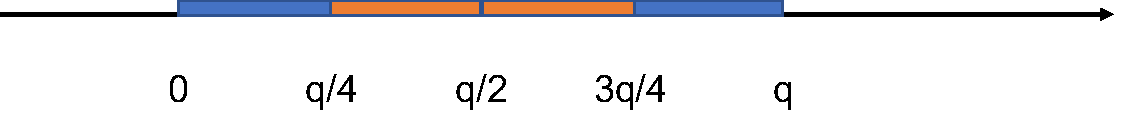
\includegraphics[width=0.9\textwidth]{error.pdf}
\end{center}
\caption{Decryption Error}
\label{error}
\end{figure}

\begin{corollary}
To compute addition $ + $(instead of XOR $\oplus$) of $k$ bit numbers $\mu_1$ and $\mu_2$, we must modify the encryption scheme by changing the factor which is multiplied with the plaintext from $\frac{q}{2}$ to $\frac{q}{2^{k+1}}$.

$$c_1 = ( \pmb{Ar_1}, \pmb{br_1} + \mu_1\floor{\frac{q}{2^{k+1}}} )$$
$$c_2 = ( \pmb{Ar_2}, \pmb{br_2} + \mu_2\floor{\frac{q}{2^{k+1}}} )$$
$$c_{add} = c_1 + c_2 = ( \pmb{A}(\pmb{r_1} + \pmb{r_2}), \pmb{b}(\pmb{r_1} +\pmb{r_2}) + (\mu_1 + \mu_2)\floor{\frac{q}{2^{k+1}}} )$$

On the basis of the similar argument described above, the error of the equations for 1 addition be 
constrained by $e_i \leq \frac{q}{2^{k+1}}$.
\end{corollary}
\begin{remark}
It is also possible to implement a similar addition for the private key encryption  scheme 
using LWE. That is, adding two ciphertexts $c_1$ and $c_2$ corresponding to $\mu_1$ and $\mu_2$
would also result in encryption of message $\mu_1 + \mu_2$.
\end{remark}

\section{Towards FHE multiplication:}
Let us try to apply a similar logic for multiplying two ciphertexts. The components of the vectors and dimensions do not check out, but we plan to investigate what happens when we try to directly multiply the ciphertexts. By multiplication of ciphertexts, we mean component-wise multiplication of the ciphertext tuple. 

$$c_1 = ( \pmb{Ar_1}, \pmb{br_1} + \mu_1\floor{\frac{q}{2}} )$$
$$c_2 = ( \pmb{Ar_2}, \pmb{br_2} + \mu_2\floor{\frac{q}{2}} )$$
$$c_{mult} = c_1 * c_2 = ( \pmb{A}\pmb{r_1} * A \pmb{r_2}, \pmb{b}\pmb{r_1} *\pmb{b}\pmb{r_2} + (\mu_1 * \mu_2)\floor{\frac{q}{2}}\floor{\frac{q}{2}} + \pmb{br_1}\mu_2\floor{\frac{q}{2}} + \pmb{br_2}\mu_1\floor{\frac{q}{2}} )$$

Again, we ask the reader to look over the fact that the dimensions in this system of equations do not. We are trying to investigate the possible problems to motivate to a possible solution.

\begin{problem}
    Applying the decryption step does not result in something clean which can be easily decrypted directly.
\end{problem}
Intuitively, we can see that the problem is there because decrypting the first term does not get rid of the noise directly. We are going investigate this problem deeper into the next lecture, but the high-level idea is to transform a ciphertext $c_2$ with an operation $G^{-1}(c_2)$ before multiplying it with $c_1$. This transformation must ensure that the values of $G^{-1}(c_2)$ are small so that the error is contained, but also must preserve the correctness of the scheme.

\section*{Acknowledgement}
These scribe notes were prepared by editing a light modification of the template designed by Alexander Sherstov.
%retain this acknowledgment in all scribe notes.

\bibliographystyle{abbrv}
\bibliography{template}

\end{document}
